\documentclass[10pt,twocolumn,letterpaper]{article}

\usepackage{cvpr}
\usepackage{times}
\usepackage{epsfig}
\usepackage{graphicx}
\usepackage{amsmath}
\usepackage{amssymb}

% Include other packages here, before hyperref.

% If you comment hyperref and then uncomment it, you should delete
% egpaper.aux before re-running latex.  (Or just hit 'q' on the first latex
% run, let it finish, and you should be clear).
\usepackage[breaklinks=true,bookmarks=false]{hyperref}

\cvprfinalcopy % *** Uncomment this line for the final submission

\def\cvprPaperID{****} % *** Enter the CVPR Paper ID here
\def\httilde{\mbox{\tt\raisebox{-.5ex}{\symbol{126}}}}

% Pages are numbered in submission mode, and unnumbered in camera-ready
%\ifcvprfinal\pagestyle{empty}\fi
\setcounter{page}{1}
\begin{document}

%%%%%%%%% TITLE
\title{Aspect Ratio Sensitive Network (ARS-Net) \\ 
\small Project Report of CS272 Computer Vision
}

\author{Jianxiong Cai\\
ShanghaiTech University\\
{\tt\small caijx@shanghaitech.edu.cn}
% For a paper whose authors are all at the same institution,
% omit the following lines up until the closing ``}''.
% Additional authors and addresses can be added with ``\and'',
% just like the second author.
% To save space, use either the email address or home page, not both
\and
Anqi Pang\\
ShanghaiTech University\\
{\tt\small pangaq@shanghaitech.edu.cn}
\and
Peijia Xu\\
ShanghaiTech University\\
{\tt\small xupj@shanghaitech.edu.cn}
\and
Lei Jin\\
ShanghaiTech University\\
{\tt\small jinlei@shanghaitech.edu.cn}
\and
Ruijian Li\\
ShanghaiTech University\\
{\tt\small lirj@shanghaitech.edu.cn}
}


\maketitle
%\thispagestyle{empty}

%%%%%%%%% ABSTRACT
\begin{abstract}
\par
Many objects in real world have a prior knowledge, which could be helpful for object detection. In this project, we propose an approach to include aspect ratio as the prior knowledge. Our approach duplicate the RPN network in faster RCNN \cite{fasterRCNN} so that different RPN can focus on generating proposal of different shapes.
\par
Our approach dramatically improves the performance (AP) of certain classes. However, our approach bring two major drawback: 1) the speed descreases as adding more RPN. 2) more false negative appear as different RPNs generate equal number of proposal for now.

\end{abstract}

%%%%%%%%% BODY TEXT
\section{Introduction}
\par
\subsection{Object Detection}
\par
General-purpose object detection on RGB images plays an important role in various applications, like autonomous driving and security. Two-stage approach like Faster RCNN \cite{fasterRCNN} shows a better performance in terms of mAP, compared with one-stage network such as YOLO.
\par
In Faster RCNN, RPN Network is used for proposing ROI regions. Lots of work has been made to refine region proposal and combine prior knowledge, which would be introduced in section \ref{sec:related-work}. In this project, we combine the prior knowledge of aspect ratio.

\subsection{Aspect Ratio (Motivation)}
\begin{figure}[h]
\centering
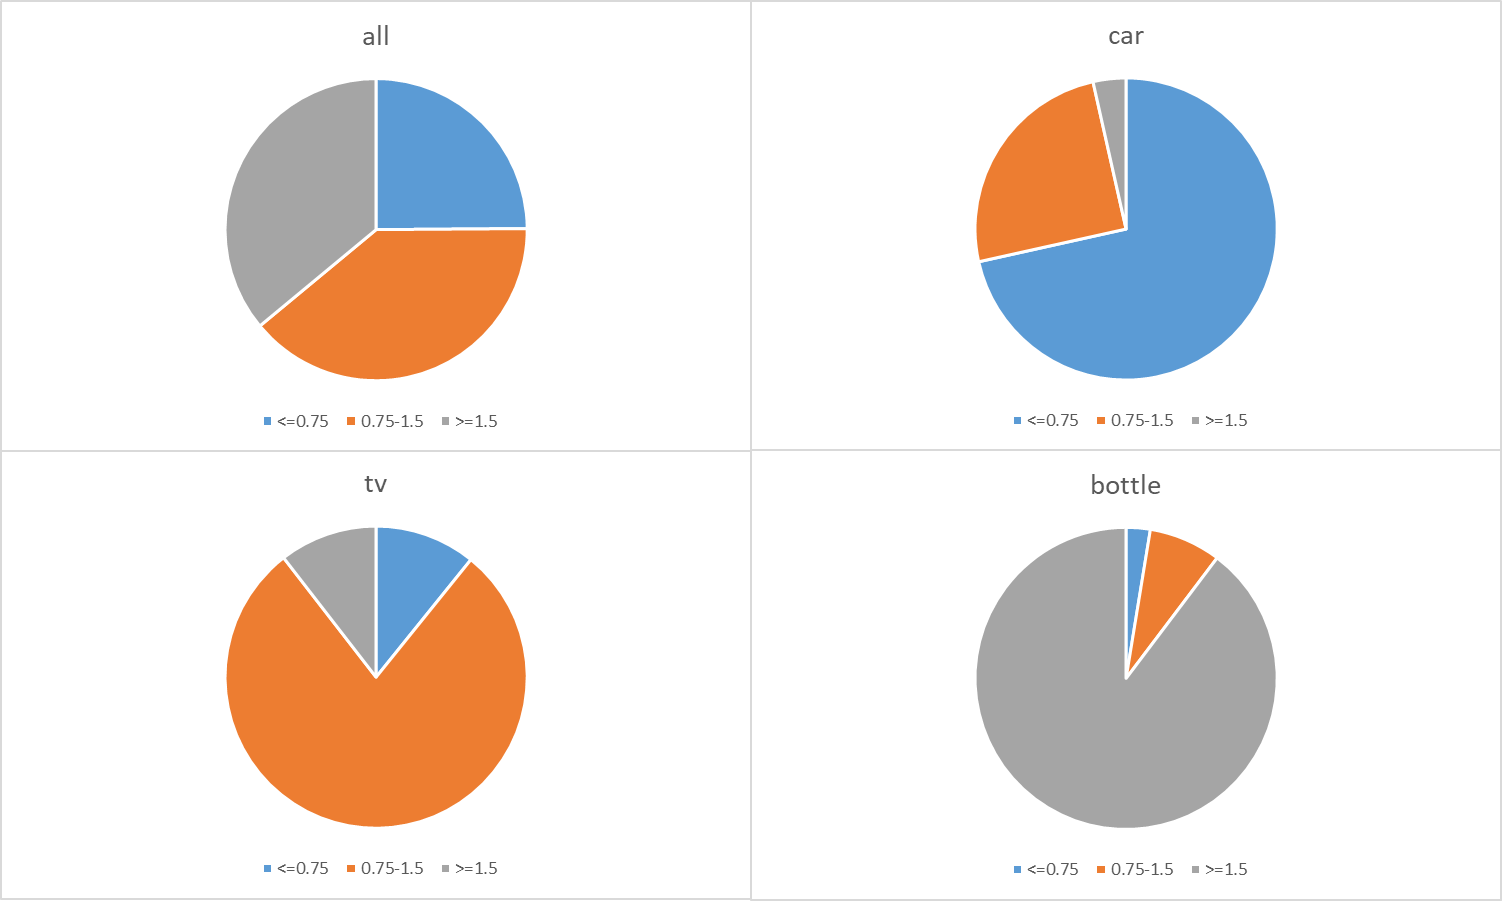
\includegraphics[width=0.7\linewidth]{pic/dist_pics/o_piescoc}
\caption{Pie charts of VOC2007}
\label{fig:piesvoc}
\end{figure}

\begin{figure}[h]
\centering
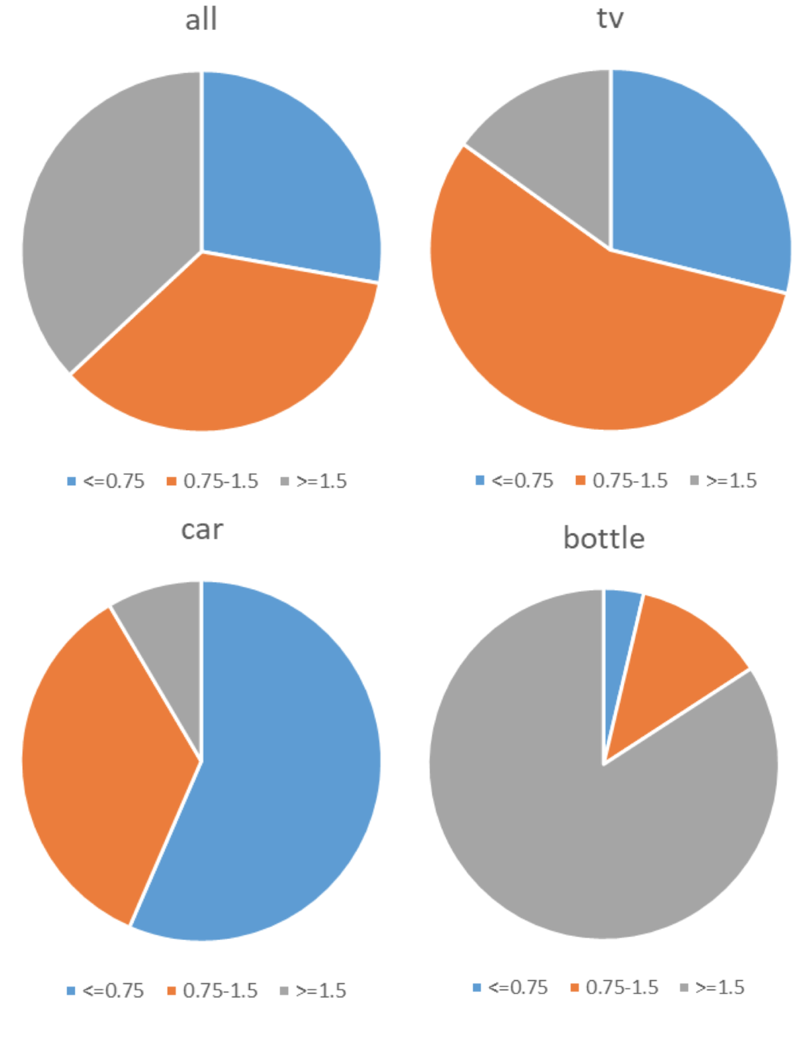
\includegraphics[width=0.7\linewidth]{pic/dist_pics/pies_coco}
\caption{Pie charts of MS COCO}
\label{fig:piescoco}
\end{figure}
% TODO: we don't need to histogram
As objects usually do not deform so much, they are generally with relatively fixed shape in some extent, which infers that the target bounding box will have certain relationship with aspect ratio especially for non-living objects. An intuitive example is that bottle will be more likely to have large aspect ratios (width to height), i.e. tall and thin. According to the statistics, both of the two commonly used datasets, VOC and MS COCO, are showing the regulation. Following histograms describe that for some classes objects are tend to be with some aspect ratios. 

% \begin{figure}[h]
% \centering
% 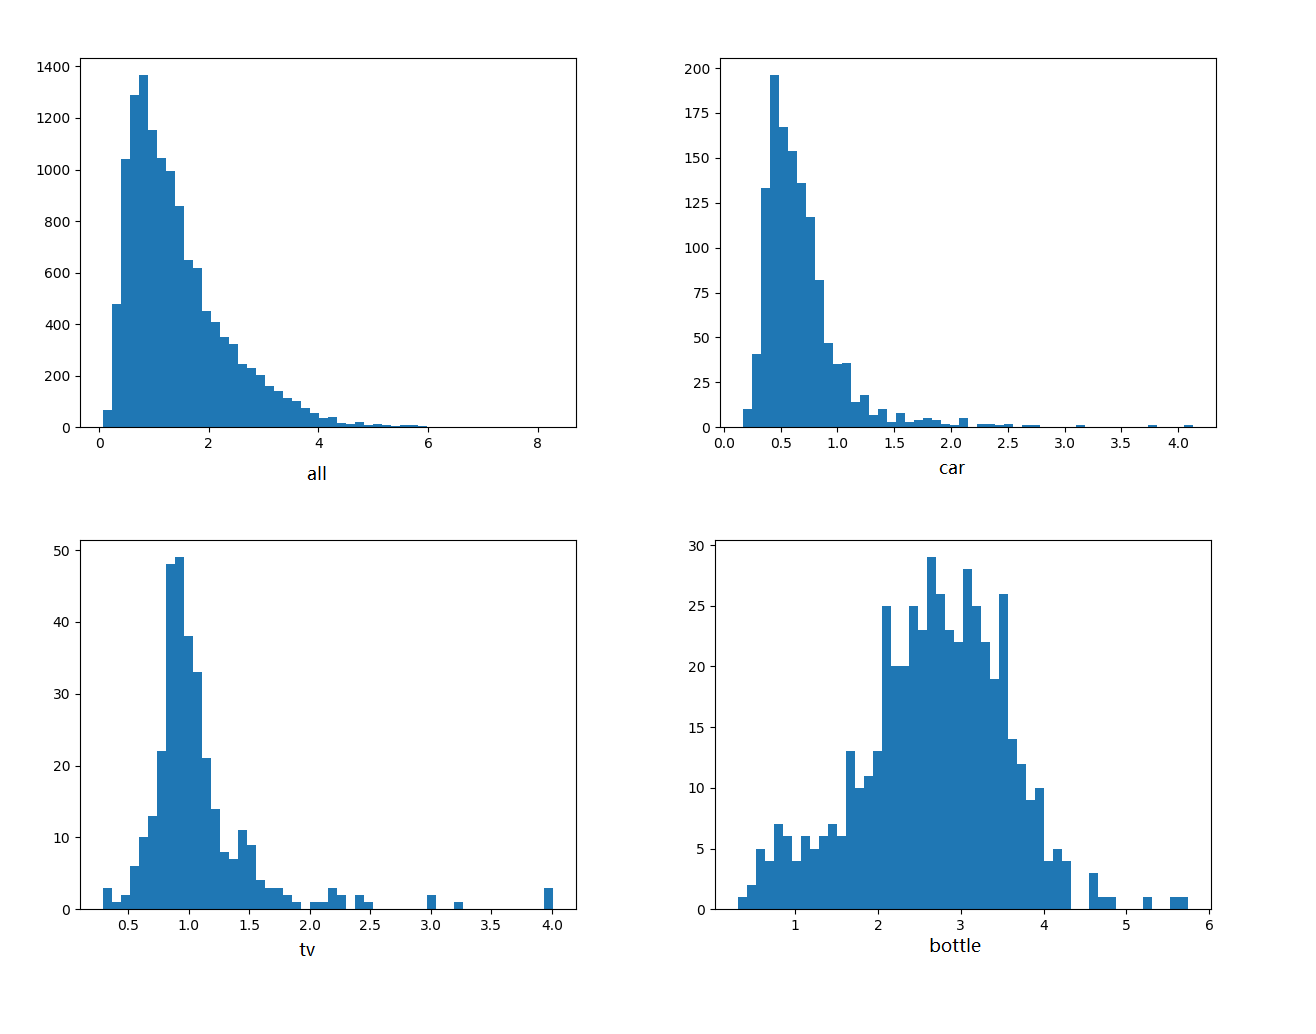
\includegraphics[width=0.7\linewidth]{pic/dist_pics/voc_hist}
% \caption{Histograms of VOC2007}
% \label{fig:vochist}
% \end{figure}

% \begin{figure}[h]
% \centering
% 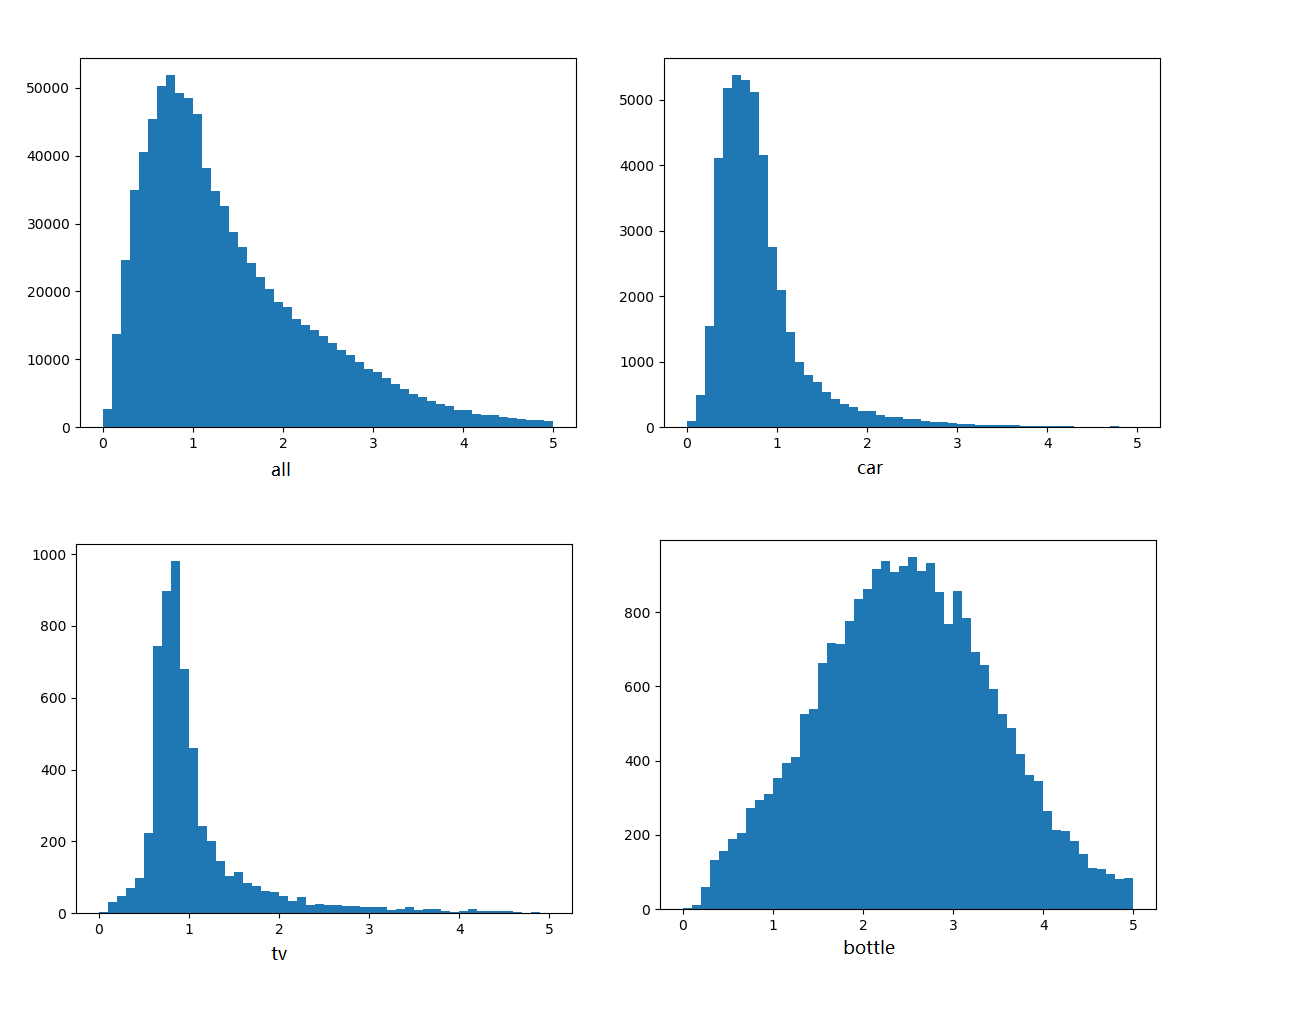
\includegraphics[width=0.7\linewidth]{pic/dist_pics/hist_coco}
% \caption{Histograms of MS COCO}
% \label{fig:histcoco}
% \end{figure}



% TODO: add cition to the fatser RCNN
The original RPN network in Faster RCNN \cite{fasterRCNN} have 3 anchor shape: 1:2, 1:1 and 2:1. Thus we count the distribution of object shape by dividing their aspect ratios into those three ratios, as is shown in fig.\ref{fig:piesvoc} and fig.\ref{fig:piescoco}.

\subsection{ARS-Net}
\begin{figure}[h]
\centering
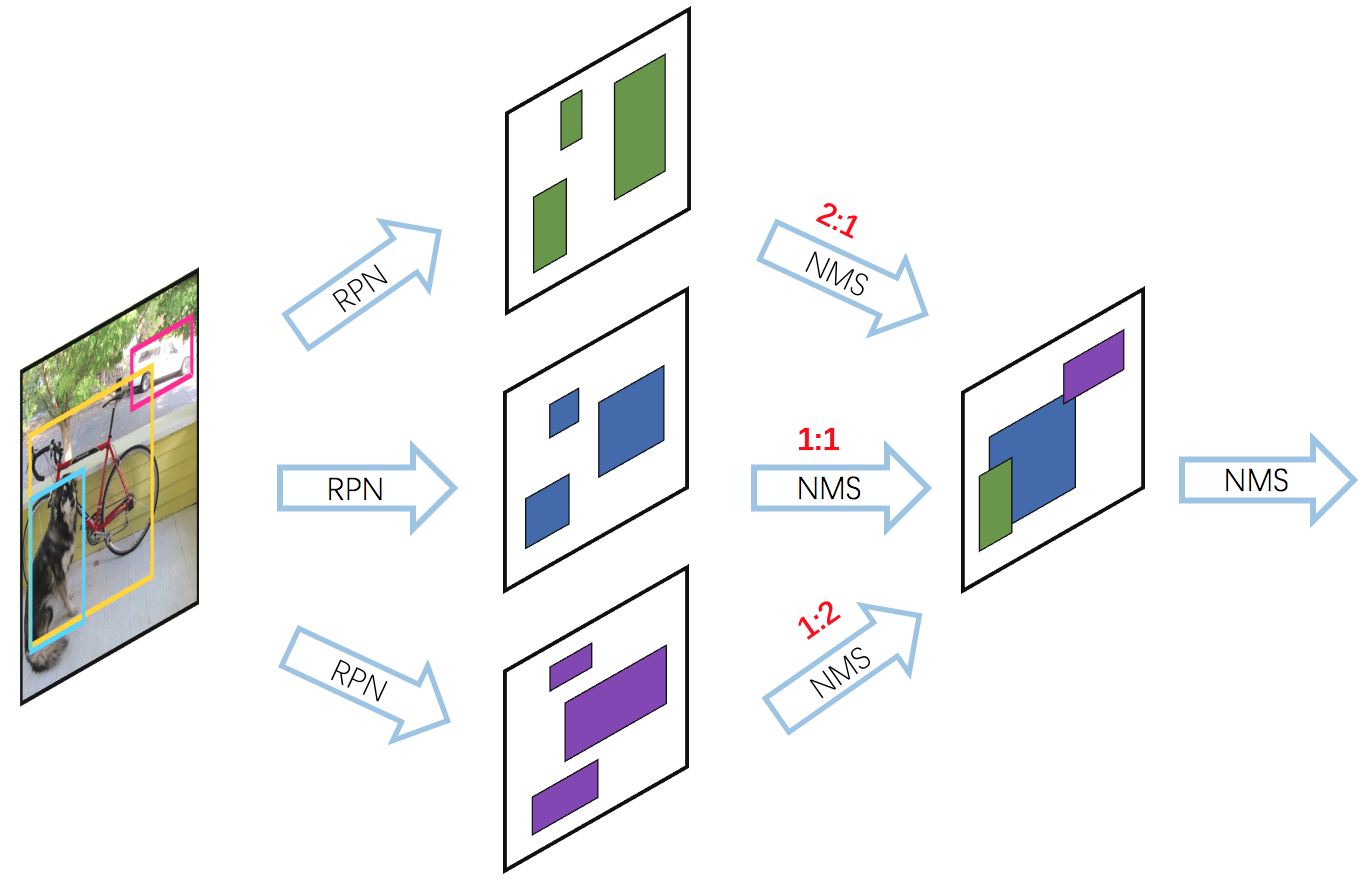
\includegraphics[width=0.7\linewidth]{pic/ARS-archi-abstract.png}
\caption{ARS-Net RPN architecture}
\label{fig:ARS-archi}
\end{figure}

\par
In this project, we propose a new approach ( as is shown in fig.\ref{fig:ARS-archi} ) to include aspect ratio as the prior knowledge for object detection. Although aspect ratio is a relatively weak feature for objects, we observes that it holds for certain object classes in most major datasets. Our approach dramatically improve the performance (AP) for those certain classes.

\section{Related Work}
	\label{sec:related-work}

\subsection{R-CNN}
~\cite{RCNN} addressed the R-CNN detector which promote the accuracy of nueral networks for object detection. This R-CNN detector combines a region proposal part (Selective Search~\cite{SelectiveSearch}), a CNN feature extractor and a classifer. R-CNN detector surmount conventional detectors in the aspect of accuracy but its speed is limited by generating massive region proposals and extracting features using CNN on each of the region proposal. 

Spatial pyramid pooling (SPP)~\cite{SPP} introduced a way to meliorate by employ pyramid pooling layer. SPP-net speed up the detector by computing CNN only once per image. Imitating SPP-net, Fast-RCNN ~\cite{fastRCNN} shown that using multi-task learning and back-propagation through ROI pooling layer will speed up the R-CNN detector by an order of magnitude. 

The bottleneck of Fast-RCNN is conventional region proposal generator, so Faster-RCNN ~\cite{fasterRCNN} proposed Region Proposal Network (RPN) which sharing features with classifer network.


\subsection{Region Proposal}
Most traditional region proposal methods are based on low-level features. Faster-RCNN introduced Region Proposal Network (RPN) to generate region proposals based on high-level semantic features. RPN surpass conventional region proposal methods, either unsupervised method (e.g. Selective Search~\cite{SelectiveSearch} and EdgeBoxes \cite{EdgeBoxes}) or supervised method (e.g. BING~\cite{BING}), on both speed and accuracy.

There are several approach of refining region proposals.

\subsubsection{cascade refinement}
Region Proposal Network can be refined by applying a multi-stage cascading pipeline structure. Applying a two-class Fast RCNN to refine proposals has shown significant improvement. \cite{CRAFT} \cite{CraftingGBD} \cite{DeepBox}.  

DeepProposal~\cite{DeepProposal} introduce a Cascading Deep Convolutional Layers to get feature maps. CascadedCNN \cite{Cascadedcnn} proposes a RefineNet added after RPN which can effectively reduce the number of proposals and improve their confidence. MTCNN~\cite{MTCNN} apply similar approach, using a R-net to refine P-net.

~\cite{GroupRecursive} introduce a spatial correlation related method, using a new EM-like group recursive learing approach to iteratively refine object proposals and provide an optimal spatial configuration of object detections.
\subsubsection{multi-scale refinment}
Methods like SDP,SSH or MS-CNN ~\cite{SDP}~\cite{SSH}~\cite{MSCNN}make independent prodictions at different layers, which will ensure smaller objects are trained on higher resolution layers.


Other methods like FPN, RetinaNet~\cite{FPN}~\cite{RetinaNet} propose a pyramidal structure to combine shallow layer with deep layer to get both high-level feature and low-level feature.

\subsection{ROI and NMS}
CoupleNet~\cite{CoupleNet} propose a two branch network of ROI after RPN to obtain both local part information and global imformation.



\section{Aspect Ratio Sensitive Object Detection}
\subsection{Aspect Ratio Sensitive Network}
% Insert an image of the different aspect ratio
We have count the sapect ratio of different classes on different dataset. All datasets contain certain classes whose aspect ratio show obvious uneven distribution among different shapes. 
% For example, in MSCOCO 2017, the majority of the ball is of the shape 1*1, only a few sample gets to 1*2 and 2*1.


\subsection{Network Architure}
\paragraph{Our approach}
To include aspect ratio as a prior knowledge for object detection, we modified the network architure by duplicating the region proposal network into 3 copies, each handling objects of different shapes. During training (see figure \ref{ARS_De}), green RPN (right) is only provided with ground truth bounding boxes of aspect ratio greater than 2:1, grey one (middle) with boxes around 1:1 only and yellow one (left) with boxes smaller than 1:2 only. Results of three region proposal networks are simply stacked together in testing time. In this way, our network is able to learn separate filters for objects of different shapes. Non-maximum suppression is applied in the end to reject high over-lapping objects. 
    \begin{figure}[!htb]
    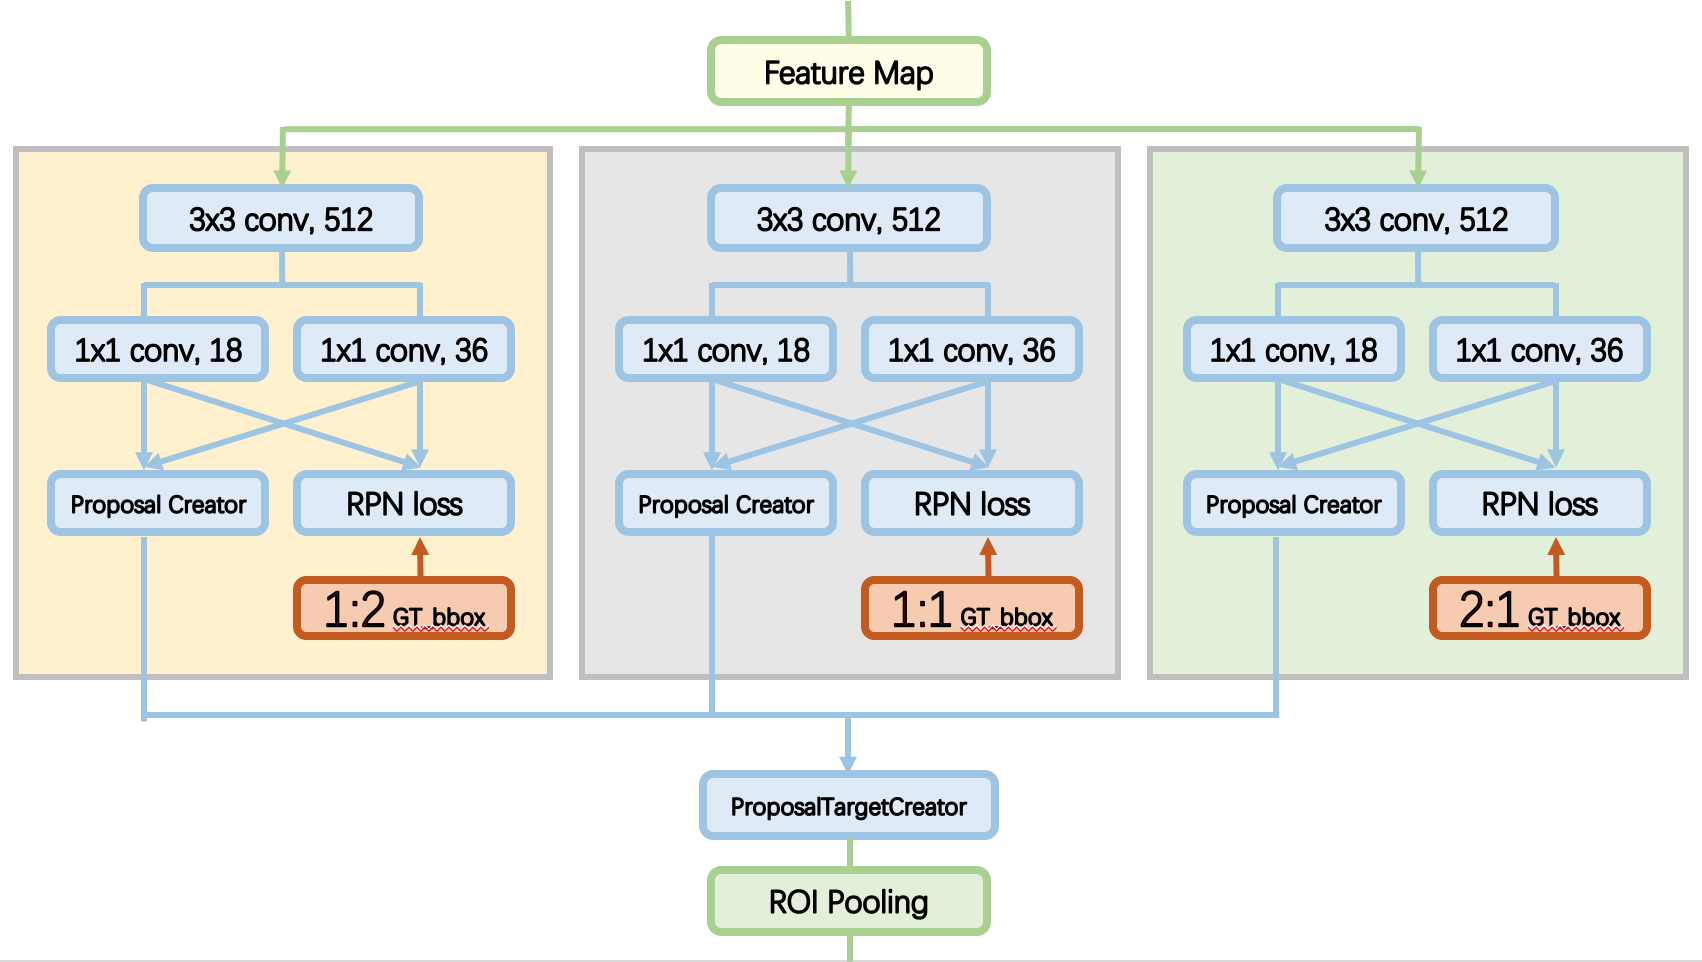
\includegraphics[width= 0.45\textwidth]{pic/ARS-archi-detail.png}
    \caption{Multiple RPN approach}
    \label{ARS_De}
    \end{figure}


\paragraph{Sharing Features}
The multi-RPN network works, but comes at great cost. One of the obvious shortcomings of this approach would be the high overall time complexity. Compared with the original faster RCNN, which runs at about 9fps on one Nvidia TitanX, our multi-RPN approach can only run at half speed. Sharing features, plus adding additional one-by-one convolutional layers are applied to cope with such problem. More specifically (see Figure \ref{ARS_sh}), three RPNs share the same 3*3*512 layer, but each would have another 1*1*256 layer of its own to further reduce depth. Other parts of the network remains unchangde. From table \ref{table_fps}, adding 1*1 conv into our network improves speed while maintaining a similar mAP. However, it's still slow when compared with the origin RCNN, afterall, region proposal network still remains to be the biggest overhead of faster RCNN.
    \begin{figure}[!htb]
    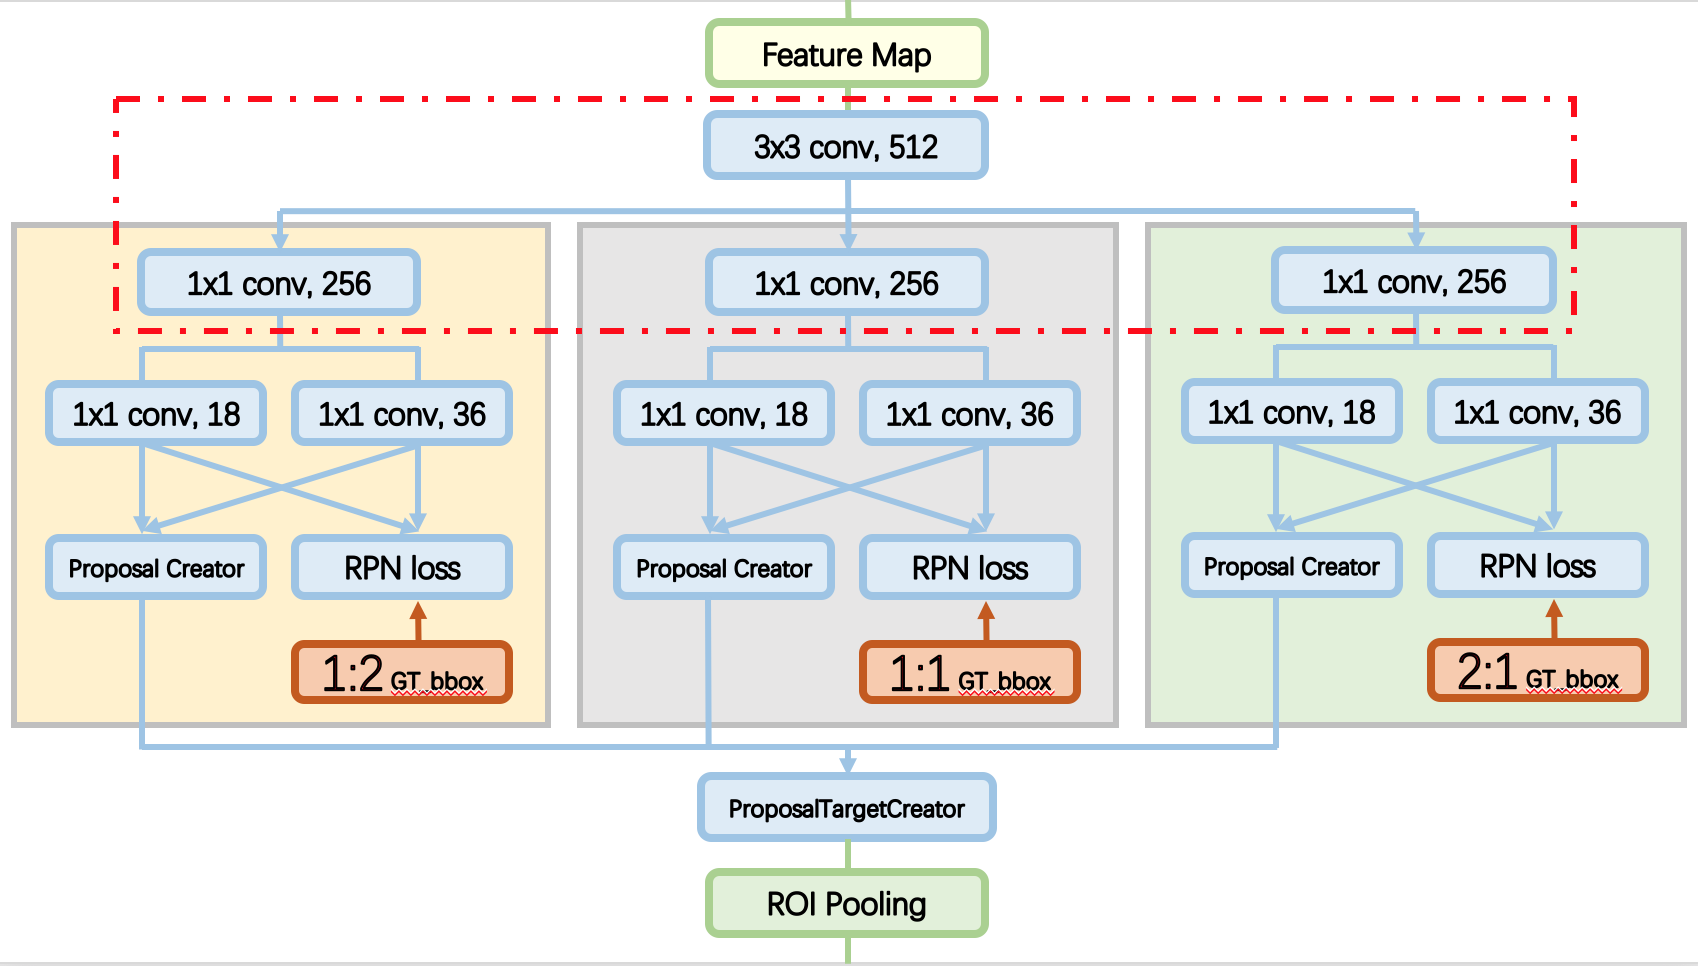
\includegraphics[width= 0.5\textwidth]{pic/ARS-archi-share.png}
    \caption{Sharing Features}
    \label{ARS_sh}
    \end{figure}

\begin{table}[ht]
\centering
\begin{tabular}{|c|c|}
\hline Approach & Frame per second \\
\hline faster RCNN (300 proposals) & 9 \\
\hline ARS-Net (300 proposals) & 4.73 \\
\hline ARS-Net (900 proposals) & 3.56 \\
\hline ARS-Net+1*1 conv (300 proposals) & 5.04 \\
\hline ARS-Net+1*1 conv (900 proposals) & 3.84 \\
\hline
\end{tabular}
\caption{Time complexity under different settings, all reported on one Nvidia TitanX. Adding 1*1 conv into our network improves speed while maintaining a similar mAP.}
\label{table_fps}
\end{table}

\subsection{Training Details}
In general, we adopted the training approaches from the origin faster RCNN. Fisrt 30 feature extraction layers are initialized with a pretrained VGG-16 model from caffe with the first 4 layers fixed, other convolutional layers are drawed from a zero-mean Gaussian distribution with standard deviation with 0.01 (\emph{REF FAST RCNN}). One single image is chosen randomly at each step to provide positive and negative samples up to 1:3 ratio for both RPNs and final classifiers. We trained the network with stochastic gradient descent (SGD) end-to-end, learning rate is set to 0.001 for the first 15 epochs. Then we fine-tuned the model with the best accuracy with another learning rate of 0.0001 for the next 15 epochs. Our approach shows an significant increase of aspect ratio sensitive class.


\begin{table*}[ht]
\label{Exp1}
\centering
\caption{Comparison}
\resizebox{\textwidth}{!}{
\begin{tabular}{l|c|c|c|cccccccccccccccccccc}
\multicolumn{1}{c|}{method} & \# of  proposals & data & mAP  & areo & bike & bird & boat & bottle & bus  & car  & cat  & chair & cow  & table & dog  & horse & mbike & person & plant & sheep & sofa & train & tv   \\ \hline

Faster RCNN      & 300 & VOC07 & 71.8 & 73.5 & 81.5 & 68.5 & 53.7 & 52.3 & 80.7 & 85.3 & 84.3 & 52.5 & 76.8 & 71.5 & 81.3 & 84.9 & 75.1 & 79.6 & 44.7 & 72.5 & 65.9 & 79.8 & 72.3 \\

ARS-Net   		  & 900 & VOC07 &\textbf{73.2}  & \textbf{74.5} & 81.5 & \textbf{71.1} & \textbf{56.7} & \textbf{56.2} & \textbf{83.6} & \textbf{85.8} & \textbf{87.4} & 51.4 & \textbf{82.7} & 68.9 & \textbf{83.8} & \textbf{86.5} & \textbf{77.1} &  \textbf{81.0} & 43.9 & \textbf{73.0} & \textbf{66.4} & 79.7 & \textbf{72.6}
\end{tabular}
\caption{Average precision of different classes reported on origin faster RCNN and out ARS-Net, highlighted ones are categories with a higher mAP}
}
\end{table*}

\section{Experiment}
\subsection{Experiments on PASCAL VOC}
We evaluate our method on the PASCAL VOC 2007 detection benchmark. This dataset consists of 5011 train images and 4952 test images over 20 object categories. Evaluation is performed on all test images. We calculated AP for each single class, and mAP at last. This is also a general metric in object detection. PR curve are also included in the end. \\
\indent{}We applied our method to Faster R-CNN with the public VGG-16 model, which has 13 convolutional layers followed by 3 fully-connected layers. Table \ref{Exp1} shows the results on VGG-16 model. Categories are highlighted if we are able to reach a better performance. Using ARS-Net, the result is 73.2\% for sharing features between proposal and detection, compared to 71.8\% that evaluated on single RPN. As shown above, our method has also dramatically improved AP in certain categories such as bottle (by 3.9\%) and cow (by 5.9\%), wich has a strong prior in shape. This is because we specify each RPN processing selected ground truth during training, which leads to the aspect ratio sensitivity. Thus the proposals generated by ARS-Net for those categories are more accurate. There's a slight decrease in several classes, which is a side effect. One possible reason is that the distribution of the test set is not consistent with the training set.

\subsection{Number of Proposals}
We further tested ARS-Net with diverse number of proposals, which is as shown in table \ref{Exp2}. When the number of proposals drops from 900 (Top 300 proposals are selected from each scale) to 300, mAP reduce by 1.7\%. And a further decrease on number of proposals leads to dropping on mAP. The main reason we thought might be that more proposals means we may have multiple proposals for a single object, where the best proposal will be selected during none maximum suppression by score. In fact, when number of proposals is 1200 in total (400 each), mAP gets a slight increase (From 73.2\% to 73.3\%). However, this change dose more harm than good. It will lead to a decrease in fps. So we take 900 proposals in total as our final result. This maintains a relatively high mAP while also taking speed into account. After using the trick of sharing features, we make ARS-Net as fast as original Faster R-CNN.

\begin{table}[ht]
\label{Exp2}
\caption{Decreasing number of proposals in ARS-Net}
\centering
\begin{tabular}{|c|c|c|}
\hline 
 method & \# of proposals & mAP
\\ \hline 
 ARS-Net & 300 & 71.5
\\ \hline 
 ARS-Net & 900 & 73.2
\\ \hline 
 ARS-Net & 1200 & 73.3
\\ \hline
\end{tabular}
\end{table}


% speed
% overall performance
\section{Things we tried but didn't work}
\par
As mentioned above, one of the major drawbacks with ARS-NEt is that it produces more false positive because the three sub-networks propose equal number of proposals. For some images, all objects may concentrate on 1*1 shape, which means all proposals from other two networks are false positive.
\par
As the result, we tried different approaches to supress those proposals.
\par 
Additionally, we want to take full advantage of aspect ratio in other parts but fail unfortunately.
\subsection{Add NMS after RPNs.}
\par
Three RPNs means more region proposal and lead more false positives in our detection results as for original faster R-CNN will decrease some RoIs in the same locations with different shapes by NMS in RPN( it might be right for some cases but not always).

\par
We simply apply NMS without score and lead mAP decrease by 0.5 roughly, decrease by 1 approximately when choose 300 RoIs after NMS. To avoid the influence caused by order, we shuffle the RoIs after stack them all together. Removing shuffle will make mAP down much more. The problem for NMS only depending on IoU may cause both false positives and negatives, as NMS can't recognize which is the right one to be left.

\par
When apply NMS with score, we face a trouble that the three RPNs are score the RoIs independently so it’s hard to make comparison and there is also a question that if the scores should be normalized so we didn’t implement the NMS with score in this step.

\subsection{Rescoring Based on Pror Distribution}
The idea to reduce score of bounding boxes with rare aspect ratios is naive. We simply multiply predicted score of the probability(calculate from the statistics of dataset) of the aspect ratio occurred in its corresponding class. It leads more than 10 decrease although the thought seems to make sense at first glance.
\par
We try to multiply the predicted score with the prior possibility and a constant k but it doesn't work as well.
\par
It failed mainly because it is almost impossible to design a rescore mapping by hand and it is not robust for extreme cases. What's more, the rightness of prior possibility is questioning.

\subsection{Cascade Head Part}
\par
All the tries can be summarized as duplicate removal indeed. The initial idea is to reshape the bounding boxes generated in the first head by prior ratio distribution to convey the class imformation to next head but fail to design a suitable reshape mapping based on aspect ratio. Then we try cascade purely but maybe some faults in programming or mistakes in traning lead that cascade method failed during training and it actually doesn't relate much about aspect ratio.
\par
We try to decrease IoU of NMS and increase the lower bound of score when implementing the second head but failed. Additionally we also try to weight the loss of different head to make the second head a more accurate classifier and regressor but fail while training.(The loss function diverges at the first epoch and then we reduce the learning rate but the mAP of the first epoch is below 10 so we quit).

\subsection{Hard-negative Mining}
We tried hard-negative mining on VOC2007 (both on original network architure and multi-RPN network). However, we didn't get obvious improvement with either network. 


\section{Discussion}
\par
Although aspect-ratio has been proved to be effective on current major datasets like VOC2007 and MSCOCO, it is relatively a weak feature for real-world objects. For example, objects like tables may show different shapes in different view-points. Some more strong features might be more effective for object detection.  

\section{Conclusion}
By including aspect ratio as a prior knowledge, our network dramatically improves performance on detecting aspect-ratio sensitive objects. However, on other object, the performance reduce because of more false positive.

\section{Contribution}
Following are contribution from each team member.
\begin{enumerate}
\item Jianxiong Cai: Training, hard-negative mining and Coordination
\item Jinglei: Multi-RPN, Training
\item Ruijian Lei
\item Peijia Xu : Dataset distribution analysis, cascade head, NMS after RPNs and rescoring(failed :( )
\item Anqi Pang : Idea, Survey Related works, some Testing and NMS and final checking.
\end{enumerate}

{\small
\bibliographystyle{ieee}
\bibliography{egbib}
}

\end{document}
